\documentclass[margin=3mm]{standalone}
\usepackage{tikz}

\begin{document}
	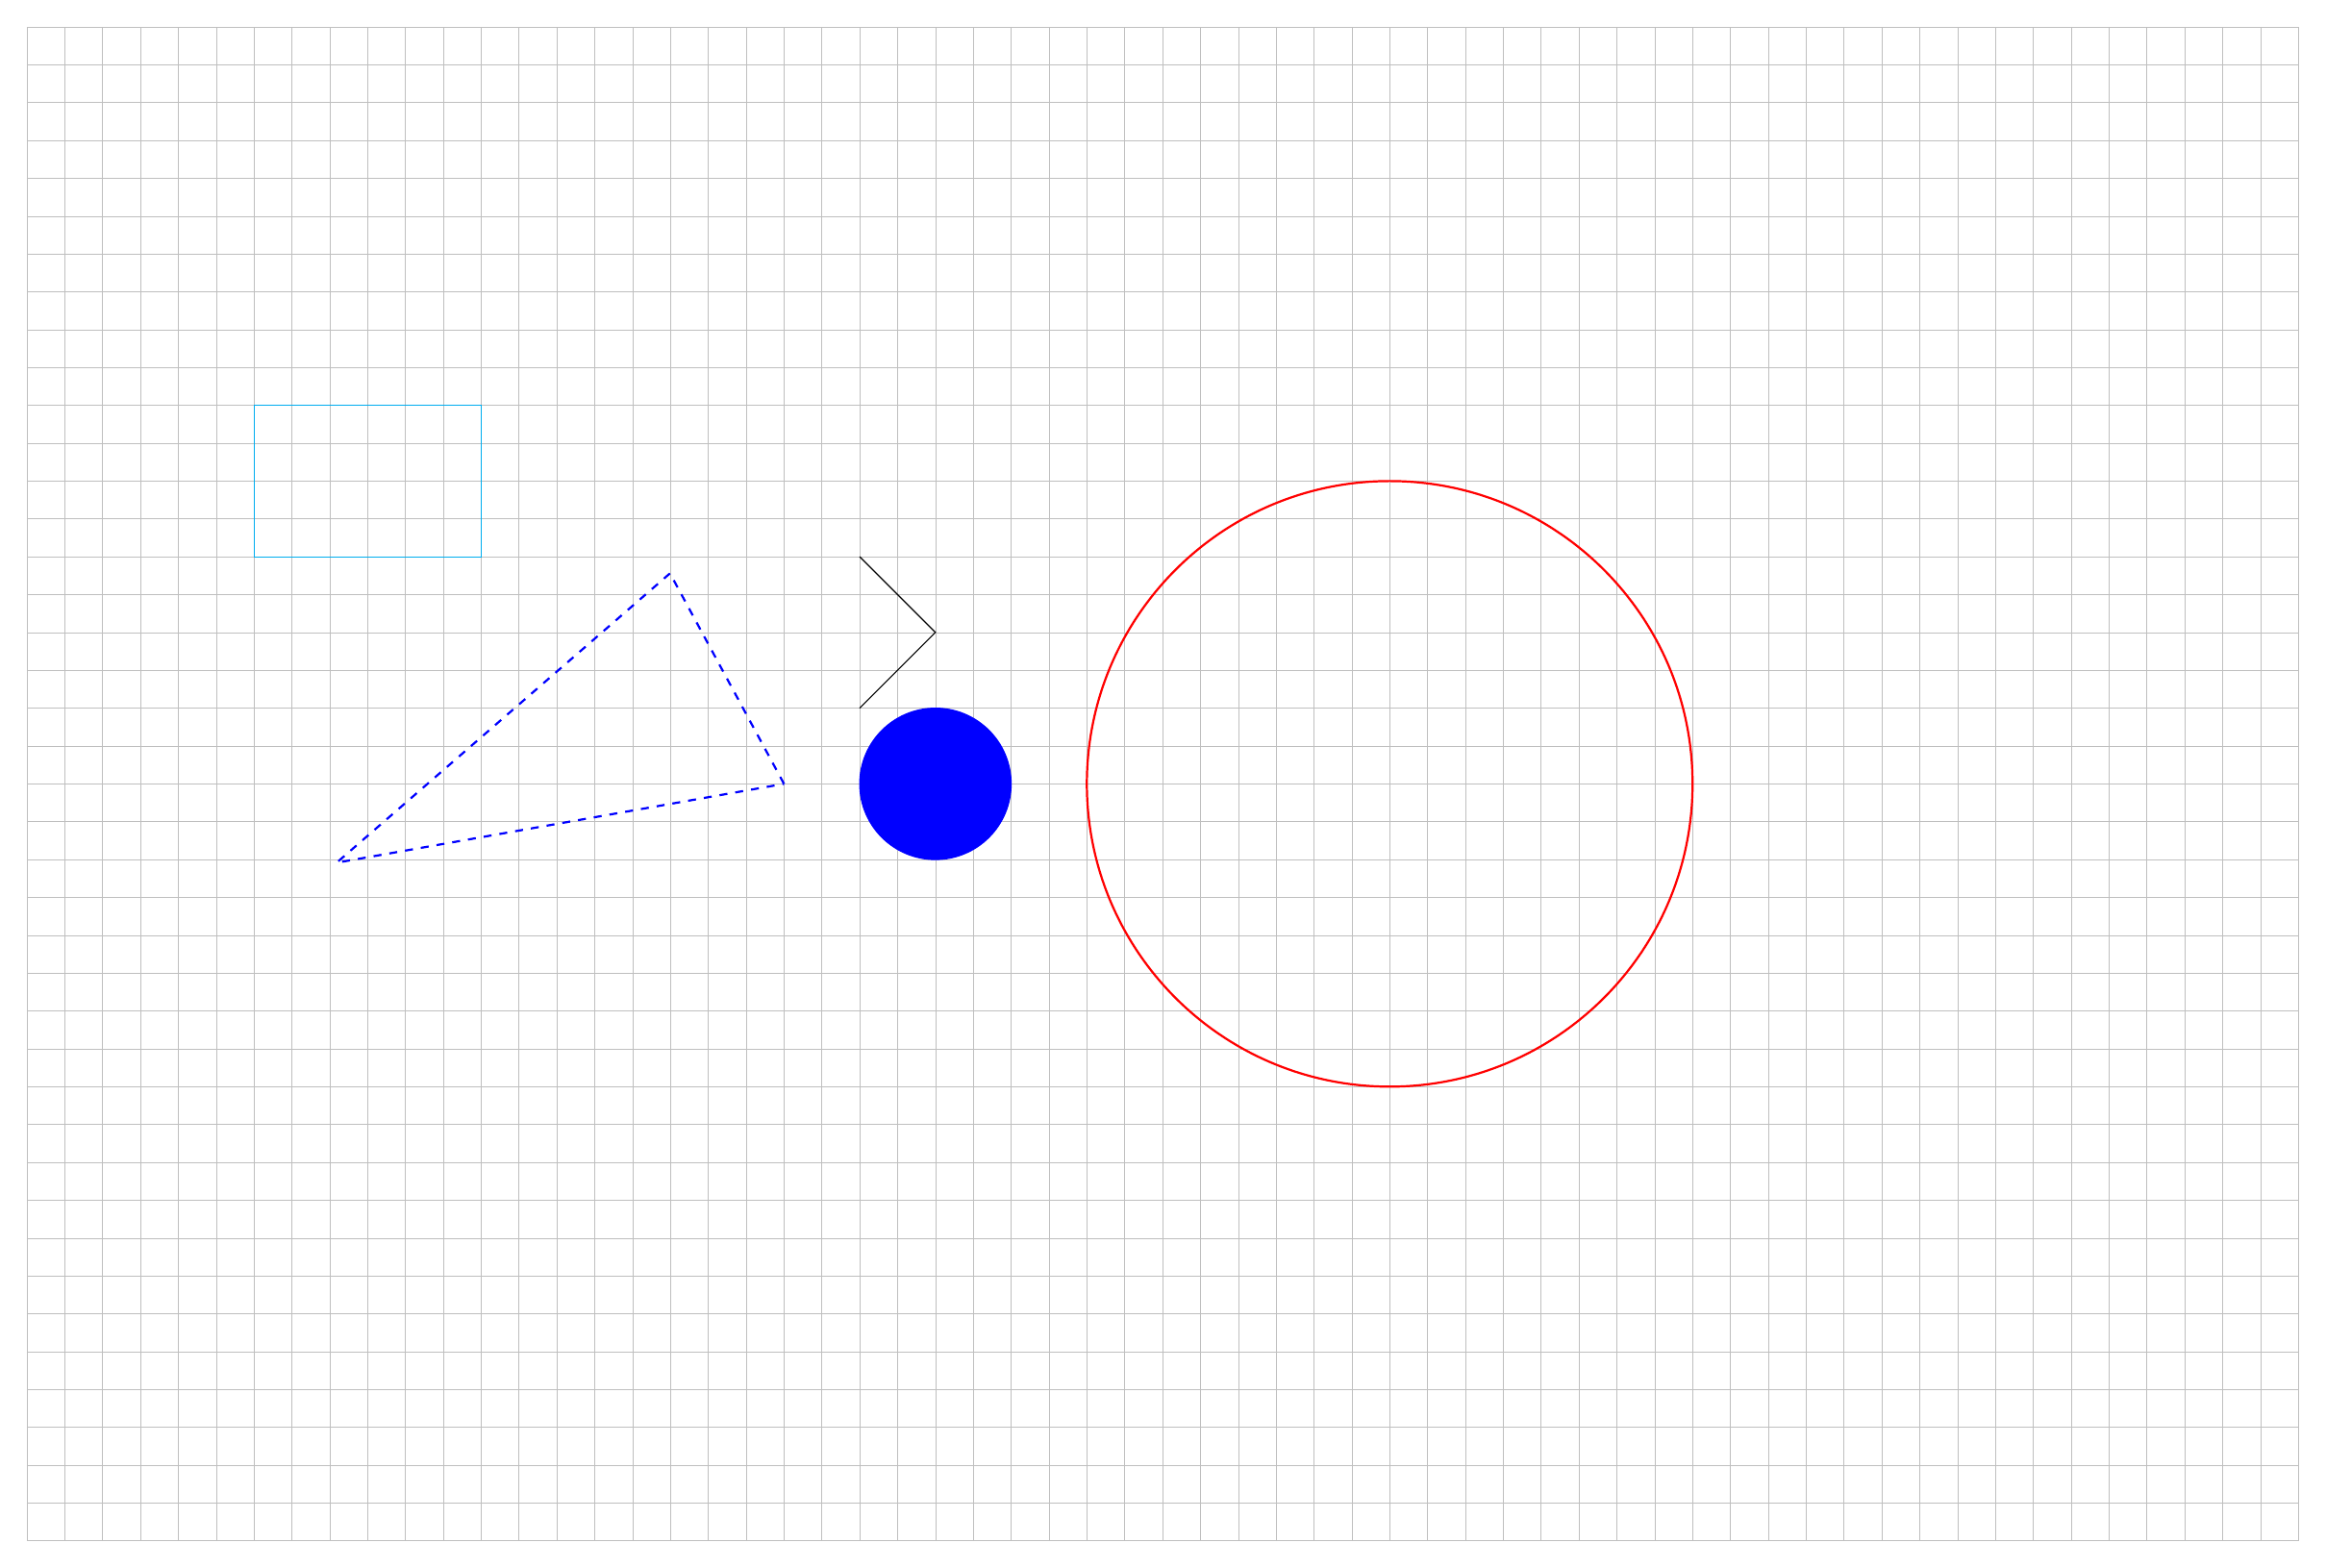
\begin{tikzpicture}
		\draw[step=0.5, gray!50, very thin](-10,-10) grid (20,10);
		\draw(1,1) -- (2,2) -- (1,3);
		\draw[blue, dashed, thick, rotate=10](0,0) -- (-1,3) -- (-6,0)--cycle;
		\draw [red, thick](8,0) circle(4);
		\draw [rotate=90,cyan](3,4) rectangle(5,7);
		\filldraw[blue] (2,0) circle (1);
		%Dibuja una elipse, se define su 
		
	\end{tikzpicture}
\end{document}